% \documentclass{beamer}
\documentclass[xcolor=dvipsnames]{beamer}
\usefonttheme{serif}
%% \usecolortheme[named=Blue]{structure}
\setbeamersize{text margin left=30mm, text margin right=30mm}
\useoutertheme{infolines}
%% \usetheme[height=7mm]{Rochester}
\usetheme{Pittsburgh}
\setbeamertemplate{items}[ball]
\setbeamertemplate{blocks}[rounded][shadow=true]
\setbeamertemplate{navigation symbols}{}

\usepackage[utf8x]{inputenc}
%% \usepackage{default}
\usepackage[english]{babel}
\usepackage{geometry}
%% \usepackage{fullpage}
\usepackage{amsmath, amsthm, amssymb}
\usepackage{listings}
\usepackage{pxfonts}
\usepackage{caption}

%% \usepackage{color}
%% \usepackage{graphicx}
%% \usepackage{natbib}
%% \usepackage{array}
%% \usepackage{booktabs}
%% \usepackage{tabu}
%% \usepackage[utf8]{inputenc}
%% \usepackage{fancyhdr}
%% \usepackage{float}
%% \usepackage{subfigure}
%% \usepackage{titlesec}

\setbeamertemplate{headline}{}
\setbeamertemplate{footline}[frame number]{}
\setbeamertemplate{navigation symbols}{}
\setbeamertemplate{footline}{}
\setbeamertemplate{footline}[frame number]

\setbeamertemplate{itemize items}{$-$}

\def\CCT{{C\nolinebreak[4]\hspace{-.05em}\raisebox{.4ex}{\tiny\bf ++}}}
\def\CC{{C\nolinebreak[4]\hspace{-.05em}\raisebox{.4ex}{\small\bf ++}}}


\definecolor{lstgray}{gray}{0.93}
\definecolor{strgray}{gray}{0.4}

\lstset{ %
  escapechar=@,
  language=C++,
  basicstyle=\footnotesize\ttfamily,
  %% basicstyle=\ttfamily,
  %% keywordstyle=\color{blue}\ttfamily,
  keywordstyle=\bfseries,
  stringstyle=\color{strgray}\ttfamily,
  commentstyle=\color{OliveGreen}\ttfamily,
  %% morecomment=[l][\color{red}]{\#},
  morecomment=[l][\color{blue}]{\#},
  backgroundcolor=\color{lstgray},
  %% keywordstyle=\color{red},
  frame=f,
  frameround=ffff,
  tabsize=2,
  breaklines=true,
  breakatwhitespace=false,
  showspaces=false,
  showstringspaces=false,
  xleftmargin=5pt,
  xrightmargin=5pt,
  morekeywords={in,out,ref,auto,inout,import,ushort,scope,exit,mixin,decltype,varid,sizeof,constexpr}
}

\def\redcolor{\color{red}}
\def\bluecolor{\color{blue}}
\def\blackcolor{\color{black}}
\def\graycolor{\color{gray}}
\def\greencolor{\color{OliveGreen}}


\def\sectionname{\translate{Section}}
\def\insertsectionnumber{\arabic{section}}
\setbeamertemplate{section page}
{
  \begin{centering}
    \begin{beamercolorbox}[sep=4pt,center]{part title}
      \usebeamerfont{section title}\insertsection\par
    \end{beamercolorbox}
  \end{centering}
}
\def\sectionpage{\usebeamertemplate*{section page}}


\AtBeginSection{\frame{\sectionpage}}


\title{Float literal}
\subtitle{A workaround}
\author{Dominic Jones}
\date{\small{November 2018}}
\institute{\small{\texttt{github.com/DominicJones}}}


\begin{document}
\begin{frame}[plain]
  \titlepage
\end{frame}


\section{From a previous talk...}


\begin{frame}[fragile]{Pruning at compile-time}
  \begin{columns}[T] % align columns
    %% \begin{column}{0.3\textwidth}
    %% \end{column}%
    %% \hfill%
    \begin{column}{0.75\textwidth}
      \begin{figure}[H]
        \centering
        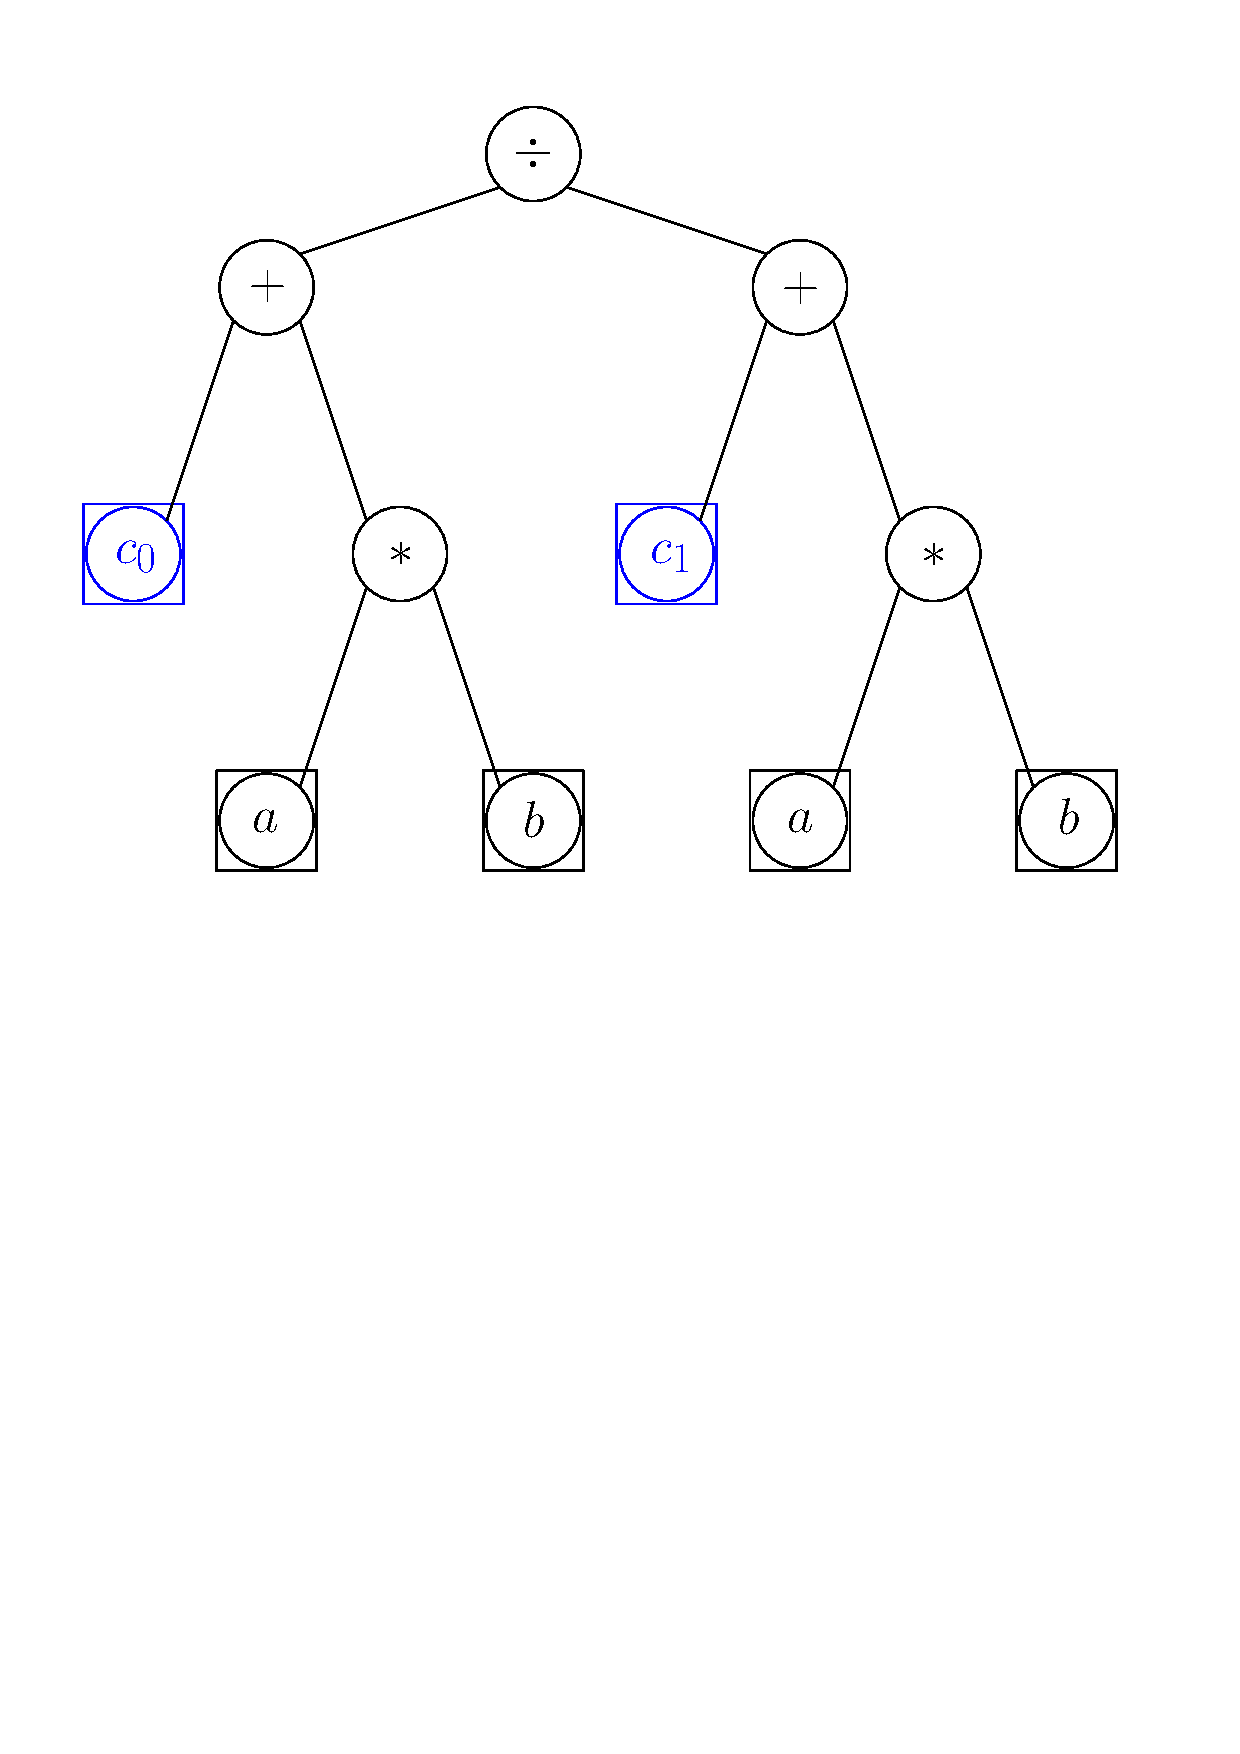
\includegraphics[width=0.99\textwidth]{fig_exprtree_cb}
      \end{figure}
    \end{column}%
  \end{columns}
\end{frame}


\begin{frame}[fragile]{Values as types}
\begin{lstlisting}
// C++ does not permit `auto' to resolve as `float'
template<auto V>
struct @\aftergroup\redcolor@_float@\aftergroup\blackcolor@
{
  constexpr operator auto() const { return V; }
};
\end{lstlisting}

~

\begin{lstlisting}
// type distinguished by value
auto constexpr @\aftergroup\bluecolor@c0@\aftergroup\blackcolor@ = -4.2@\aftergroup\redcolor@_f@\aftergroup\blackcolor@;
static_assert(@\aftergroup\bluecolor@c0@\aftergroup\blackcolor@ == @\aftergroup\redcolor@_float@\aftergroup\blackcolor@<-4.2>{});
\end{lstlisting}
\end{frame}


%% @\aftergroup\bluecolor@c1@\aftergroup\blackcolor@

\begin{frame}[fragile]{Identifiers as types}
\begin{lstlisting}
@\aftergroup\graycolor@ 1234567@\aftergroup\bluecolor@8@\aftergroup\graycolor@9 123456789 12345
         10        20
1
2  // main.cpp
@\aftergroup\bluecolor@3@\aftergroup\graycolor@@\aftergroup\blackcolor@  auto @\aftergroup\bluecolor@c1@\aftergroup\blackcolor@ = rand();@\aftergroup\graycolor@
4@\aftergroup\blackcolor@  auto constexpr loc = @\aftergroup\redcolor@&@\aftergroup\blackcolor@@\aftergroup\bluecolor@c1@\aftergroup\blackcolor@@\aftergroup\redcolor@@\aftergroup\blackcolor@;@\aftergroup\graycolor@
\end{lstlisting}


\begin{lstlisting}
@\aftergroup\redcolor@&@\aftergroup\blackcolor@@\aftergroup\bluecolor@c1@\aftergroup\blackcolor@@\aftergroup\redcolor@@\aftergroup\blackcolor@ := @\aftergroup\redcolor@hash(row, column, filename)@\aftergroup\blackcolor@
    := @\aftergroup\redcolor@hash(@\aftergroup\bluecolor@__LINE__@\aftergroup\redcolor@, @\aftergroup\bluecolor@8@\aftergroup\redcolor@, @\aftergroup\greencolor@__FILE__@\aftergroup\redcolor@)
\end{lstlisting}

~

\begin{lstlisting}
// type distinguished by location
template<typename L, typename R>
auto operator+(L const &@\aftergroup\bluecolor@l@\aftergroup\blackcolor@, R const &@\aftergroup\bluecolor@r@\aftergroup\blackcolor@)
-> Binary<Add, L, R, @\aftergroup\bluecolor@@\aftergroup\redcolor@&@\aftergroup\bluecolor@l@\aftergroup\blackcolor@, @\aftergroup\bluecolor@@\aftergroup\redcolor@&@\aftergroup\bluecolor@r@\aftergroup\blackcolor@>
{
  return {@\aftergroup\bluecolor@l@\aftergroup\blackcolor@, @\aftergroup\bluecolor@r@\aftergroup\blackcolor@};
}
\end{lstlisting}
\end{frame}


\section{In another world...}


\begin{frame}[fragile]{D programming language}
\begin{lstlisting}
// exactly what is wanted
struct Literal(@\aftergroup\bluecolor@float@\aftergroup\blackcolor@ V)
{
  static immutable auto value = V;
}
\end{lstlisting}

~

\begin{lstlisting}
// f-p constant folding is done in real or greater precision.
// Follows IEEE 754 rules and round-to-nearest is used.
static assert(Literal!(@\aftergroup\redcolor@9.0/3@\aftergroup\blackcolor@).value ==
              Literal!(@\aftergroup\redcolor@6.0/2@\aftergroup\blackcolor@).value);
\end{lstlisting}
\end{frame}


\section{Back to {C++}}


\begin{frame}[fragile]{Why cannot this be done in \CC?}
  \begin{itemize}
  \item \emph{I don't really know} \vspace{5mm}
  \item ``Two floats that are logically identical might not result in the same bit pattern, thus you would generate different templates.'' \vspace{5mm}
  \item ``The problem is that the textual representations of floating point values (constexpr) do not necessarily have the same value on different systems. And two different textual representations may map to the same value on some platforms, and different values on others.'' \vspace{5mm}
  \item ``NaN values have the curious property that they compare as `unordered' with all values, even with themselves.'' \vspace{5mm}
  \end{itemize}
\end{frame}


\begin{frame}[fragile]{Is there a workaround?}
  \begin{itemize}
  \item Yes, \vspace{5mm}
  \item if you have compile-time time for it \vspace{5mm}
  \item if compile-time programming is your favourite pastime \vspace{5mm}
  \end{itemize}
\end{frame}


\section{A rough sketch}


\begin{frame}[fragile]{``\texttt{\_float}'' type}
\begin{lstlisting}
// only fixed-point here...
template<auto H, auto L, auto E>
struct _float
{
  auto constexpr static value =
    (H + @\aftergroup\bluecolor@float@\aftergroup\blackcolor@(L) / multiplier<10, E, 1>::value);

  constexpr operator auto() const { return value; }
};
\end{lstlisting}

~

\begin{lstlisting}
// and for operator+
template<auto H, auto L, auto E>
auto constexpr operator-(_float<H, L, E>)
{
  return _float<(-H), (-L), E>{};
}
\end{lstlisting}
\end{frame}


\begin{frame}[fragile]{made palatable}
\begin{lstlisting}
// makes life easier
template<char...> struct mp_chars {};
\end{lstlisting}

~

\begin{lstlisting}
// user-defined literal
template<char... Cs>
auto constexpr operator""@\aftergroup\bluecolor@_f@\aftergroup\blackcolor@()
{
  return make_float_t<0, 0, 0, 0,
                      sizeof...(Cs), mp_chars<Cs...> >{};
}
\end{lstlisting}

~

\begin{lstlisting}
// seamless conversion to literals
auto constexpr v = -4.2@\aftergroup\bluecolor@_f@\aftergroup\blackcolor@;
float w = 2 * v;
\end{lstlisting}
\end{frame}


\begin{frame}[fragile]{Parsing}
\begin{lstlisting}

  123.45@\aftergroup\bluecolor@_f@\aftergroup\blackcolor@

  // represented as
  mp_chars<'1', '2', '3', '.', '4', '5'>

  H = '1', '2', '3'  // high chars
  L = '4', '5'       // low chars
  E = 4              // decimal offset
  N = 6              // length

\end{lstlisting}
\end{frame}


\begin{frame}[fragile]{Terminal}
\begin{lstlisting}
// all chars consumed
template<auto H, auto L, auto E,
         auto I, auto N,
         template<char...> class CL>
struct make_float<H, L, E, I, N, CL<> >
{
  using type = _float<H, L, (N - E)>;
};
\end{lstlisting}
\end{frame}


\begin{frame}[fragile]{Decimal offset}
\begin{lstlisting}
// specialise for decimal character
template<auto H, auto L, auto E,
         auto I, auto N,
         template<char...> class CL, char... Cs>
struct make_float<H, L, E, I, N, CL<'.', Cs...> >
{
  auto static constexpr _E = I + 1;
  using type = make_float_t<H, L, _E, (I+1), N, CL<Cs...> >;
};
\end{lstlisting}
\end{frame}


\begin{frame}[fragile]{Digits}
\begin{lstlisting}
// distinguish high from low by decimal offset
template<auto H, auto L, auto E,
         auto I, auto N,
         template<char,char...> class CL, char C, char... Cs>
struct make_float<H, L, E, I, N, CL<C, Cs...> >
{
  auto static constexpr _D = (C >= '0' && C <= '9');
  auto static constexpr _H = (_D && E == 0)? 10*H+(C-'0'): H;
  auto static constexpr _L = (_D && E  > 0)? 10*L+(C-'0'): L;

  using type = make_float_t<_H, _L, E, (I+1), N, CL<Cs...> >;
};
\end{lstlisting}
\end{frame}


\begin{frame}[fragile]{\texttt{if constexpr}?}
  \begin{itemize}
  \item Tried it initially \vspace{5mm}
  \item Works too well! Either perfect or uncompilable \vspace{5mm}
  \item Far easier to iteratively get something working \vspace{5mm}
  \item Perhaps rewrite once parser is completed \vspace{5mm}
  \end{itemize}
\end{frame}


\begin{frame}[plain]
  \titlepage
\end{frame}
\end{document}
